\documentclass[11pt]{article}
\usepackage{geometry}                % See geometry.pdf to learn the layout options. There are lots.
\geometry{a4paper}                   % ... or a4paper or a5paper or ... 
%\geometry{landscape}                % Activate for for rotated page geometry
%\usepackage[parfill]{parskip}    % Activate to begin paragraphs with an empty line rather than an indent
\usepackage{graphicx}
\usepackage{amssymb}
\usepackage{amsmath}
\usepackage{lipsum}
\usepackage{authblk}
%\usepackage{amsaddr}
\usepackage{epstopdf}
\usepackage{booktabs}
\usepackage{xcolor}
\usepackage{fancyhdr}
\usepackage[yyyymmdd,hhmmss]{datetime}
\pagestyle{fancy}
\rfoot{Compiled on \today\ at \currenttime}
\cfoot{}
\lfoot{Page \thepage}
\RequirePackage[colorinlistoftodos,prependcaption,textsize=tiny]{todonotes} % look for '\todo'
\definecolor{darkred}{rgb}{0.4,0.0,0.0}
\definecolor{darkgreen}{rgb}{0.0,0.4,0.0}
\definecolor{darkblue}{rgb}{0.0,0.0,0.4}
\usepackage[bookmarks,linktocpage,colorlinks,
    linkcolor = darkred,
    urlcolor  = darkblue,
    citecolor = darkgreen]{hyperref}

%\DeclareGraphicsRule{.tif}{png}{.png}{`convert #1 `dirname #1`/`basename #1 .tif`.png}

\renewcommand{\headrulewidth}{0pt}
\fancyhead[L]{
%\includegraphics[width=4cm]{/Users/tomluu/Research/talks/fzjTemplate/uniBonn_logo.jpg}
}
\fancyhead[R]{
%\includegraphics[width=4cm]{/Users/tomluu/Research/talks/fzjTemplate/fzj_logo.jpg}
}
\pagestyle{plain}

\title{SU(3) interpolating operators}
\author[1,2]{Thomas Luu}
\affil[1]{Institute for Advanced Simulation 4\\
Forschungszentrum J\"ulich, Germany}
\affil[2]{Rheinische Friedrich-Williams-Universit\"at Bonn, Germany}

%\email{t.luu@fz-juelich.de}
\date{}                                           % Activate to display a given date or no date


\begin{document}
\maketitle
\begin{center}
email: \href{mailto:t.luu@fz-juelich.de}{t.luu@fz-juelich.de}
\end{center}
\abstract{
Here I provide notes on how to construct interpolating operators at the SU(3) flavor symmetric point.  In particular, I consider the two-meson system, where one of the mesons is a $D$-meson with a light quark (at the SU(3) point), and the other is an octet meson at the SU(3) point.
}

\thispagestyle{fancy}

\clearpage{}
%\tableofcontents
%\newpage

\section{Setup}
Since the $D$-meson has a charm quark that has no flavor, its representation is given by the light anti-quark, which is $[\bar 3]$.  I want to combine this with a light meson that falls in the $[8]$ representation.  Group theory gives (I don't remember how to actually do this!)
\begin{displaymath}
[\bar 3]\otimes[8]=[15]\oplus[6]\oplus[\bar 3]\ .
\end{displaymath}
The $[15]$ rep is repulsive, the $[\bar 3]$ is attractive, and $[6]$ is somewhere inbetween.  I want to investigate the $[\bar 3]$ and $[6]$ representations on the lattice.  So I need to figure out how to construct interpolating operators that fall into these irreps.

\section{Interpolating operators for the D-meson}
The (local) interpolating operator at position $x$ (4-vector) for the $D$-meson is simplest to deal with, and so I start with it:
\begin{equation}\label{eqn:D interp}
\psi_D^f(x)= \bar{q}_{a,\alpha}^f(x)[\Gamma]_{\alpha\beta}c_{a,\beta}^{}(x)\equiv  \bar{q}_{a}^f(x)\Gamma c_{a}^{}(x)\ ,
\end{equation}
where 
\begin{equation}\label{eqn:Gamma}
\Gamma=
\begin{cases}
\gamma_5\quad\quad\text{pseudoscalar}\\
\gamma_i\quad\quad\text{vector}
\end{cases}\ ,
\end{equation}
$c$ is the charm quark operator, $\bar{q}$ the light anti-quark operator, the index $a$ refers to color charges, $\alpha$ and $\beta$ are spinor indices\footnote{In these notes I use Greek letters for spinors and Roman letters for color.  I suppress spinor indices as much as possible.} and $f$ refers to the remaining quantum numbers of the light anti-quark, i.e. the hypercharge $Y$ (strangeness, $=0,1$), isospin $I$ ($=0,1/2)$, and isospin projection $I_z$ ($=0,\pm1/2$).    There are also the quadratic Casimir ($C_1$) and cubic Casimir ($C_2$) eigenvalues, which for the $[\bar 3]$ (where $\bar q$ resides), are $4/3$ and $10/9$ (check!!), respectively.  The form of the operator ensures that this object is a color singlet. 

\section{Coupling $c[\bar{3}]\otimes [3]\otimes[\bar{3}]$}
For the time being I ignore the spinor degrees of freedom, i.e. I omit the $\Gamma$ matrix from Eq.~\eqref{eqn:Gamma} from my calculations.  I will insert this back in later.  Group theory gives (I drop the charm quark label, as it just tags along)
\begin{equation}
[\bar{3}]\otimes [3]\otimes[\bar{3}]=[\bar{3}]\otimes ([{\color{blue} 8}]\oplus[{\color{red}1}])
=[{\color{blue}15}]\oplus[{\color{blue}6}]\oplus[{\color{blue}\bar{3}}]\oplus[{\color{red}\bar{3}}]\ .
\end{equation}
I will not consider the $[{\color{red}\bar{3}}]$ states, as this is simply the direct product of the light anti-quark of the D-meson with the singlet $q\bar{q}$ state (which has lots of disconnected diagrams!), and is not of interest in these calculations.

\subsection{Tensor method of H. Georgi}
Here I use the tensor formalism given in Georgi's book (\texttt{Lie Algebra in Particle Physics}, chapter 10)\footnote{Thanks Christoph for pointing this out to me!}.  Lower tensors ([3]), for example, are defined as
\begin{displaymath}
\left. \begin{array} { l } { | 1 / 2 , \sqrt { 3 } / 6 \rangle \left. \equiv \right| _ { 1 } \rangle } \\ { | - 1 / 2 , \sqrt { 3 } / 6 \rangle \left. \equiv \right| _ { 2 } \rangle } \\ { | 0 , - 1 / \sqrt { 3 } \rangle \left. \equiv \right| _ { 3 } \rangle } \end{array} \right.
\end{displaymath}
General lower tensor transforms as
\begin{displaymath}
\left. T _ { a } \right| _ { i } \rangle =\left. \right| _ { j } \rangle \left[ T _ { a } \right] _ { i } ^ { j }
\end{displaymath}
where $T_a=\frac{1}{2}\lambda_a$ are related to the Gell-Mann SU(3) matrices ($a=1\ldots 8$).
One has similar definitions for upper tensors ([$\bar{3}$]).

A general tensor is defined as
\begin{displaymath}
\left.\right| _ { j _ { 1 } \cdots j _ { n } } ^ { i _ { 1 } \cdots i _ { m } } \rangle =|_{j_1}\rangle\cdots|_{j_n}\rangle\otimes
|^{i_1}\rangle\cdots|^{i_m}\rangle
\end{displaymath}
and transforms as
\begin{align*}
\left[ T _ { a } \right]\left.\right| _ { j _ { 1 } \cdots j _ { n } } ^ { i _ { 1 } \cdots i _ { m } } \rangle =& \sum _ { \ell = 1 } ^ { \infty }\left.\right| _ { j _ { 1 } \cdots j_{\ell-1}, k,  j_{\ell+1}\cdots j _ { n } } ^ { i _ { 1 } \cdots i _ { m } } \rangle 
\left[ T _ { a } \right] _ { j _ { \ell } } ^ { k } \\
-&\sum _ { \ell = 1 } ^ { \infty }\left.\right| _ { j _ { 1 } \cdots j _ { n } } ^ { i _ { 1 } \cdots i_{\ell-1}, k,  i_{\ell+1}\cdots i _ { m } } \rangle 
\left[ T _ { a } \right] _ { k } ^ { i_\ell }
\end{align*}

A general vector in this space is
\begin{displaymath}
| v \rangle =\left.\right| _ { j _ { 1 } \cdots j _ { n } } ^ { i _ { 1 } \cdots i _ { m } } \rangle v _ { i _ { 1 } \cdots i _ { m } } ^ { j _ { 1 } \cdots j _ { n } }
\end{displaymath}
This defines the tensor \emph{component}.  Tensor \emph{products} of components are
\begin{displaymath}
[ u \otimes v ] _ { j _ { 1 } \cdots j _ { m } j _ { 1 } ^ { \prime } \cdots j _ { q } ^ { \prime } } ^ { i _ { 1 } \cdot i_n\ i'_1 \cdots i_ { p } ^ { \prime } } = u _ { j _ { 1 } \cdots j _ { m } } ^ { i _ { 1 } \cdots i _ { n } } v _ { j _ { 1 } ^ { \prime } \cdots j _ { q } ^ { \prime } } ^ { i _ { 1 } ^ { \prime } \cdots i _ { p } ^ { \prime } }
\end{displaymath}
We can build up our SU(3) basis states from such tensor component products, and their transformation properties are dictated by $T_a$.  {\color{red} To get the states to fall into definite $(n,m)$ irreps, one must \emph{project}!}

\subsection{Projection operators}
The relevant tensor component space in our problem is $[u\otimes\mu\otimes\nu]^{i,j}_k=u^i\mu^j\nu_k\equiv u^iv^j_k$. 
Again, following Georgi's book, I can determine the projection operators and I list the relevant ones for our case here:
\begin{align*}
P[{\color{red}\bar{3}}]^{ij}_k&=\frac { 1 } { 3 } \left( \delta _ { k } ^ { j } u ^ { i } v _ { \ell } ^ { \ell }  \right)\\
P[{\color{blue}\bar{3}}]^{ij}_k&=\frac { 1 } { 8 } \left( 3 \delta _ { k } ^ { i } u ^ { \ell } v _ { \ell } ^ { j } - \delta _ { k } ^ { j } u ^ { \ell } v _ { \ell } ^ { i } \right)\\
P[{\color{blue}6}]^{ij}_k&=- \frac { 1 } { 4 } \epsilon ^ { i j \ell } \left( \epsilon _ { \ell m n } u ^ { m } v _ { k } ^ { n } + \epsilon _ { k m n } u ^ { m } v _ { \ell } ^ { n } \right)\\
P[{\color{blue}15}]^{ij}_k&=1-P[{\color{red}\bar{3}}]^{ij}_k-P[{\color{blue}\bar{3}}]^{ij}_k-P[{\color{blue}6}]^{ij}_k\ .
\end{align*}
The procedure to construct states of definite irrep symmetry is now standard.  I diagonalize these projection operators in the basis of states.  The eigenvalues should either be 1 or 0, the former giving eigenstates that provide the correct linear combinations of the states for the irrep in question.  The states in the $[\bar{3]}$, $[6]$, and $[15]$ representations are given in~\autoref{tab:3b},~\autoref{tab:6}, and~\autoref{tab:15}, respectively.

\begin{table}
\center
\caption{The states in the $[{\color{blue}\bar{3}}]$ representation and their associated quantum numbers.  $T^2_a$ is the Casimir operator, $I_z$ is the third component of isospin, and $Y$ is the hypercharge.\label{tab:3b}}
\begin{tabular}{c|c|c|c|c}
state&components & $T_a^2$ & $I_z$ & $Y$\\
\hline\hline
1&$|1\rangle|\bar{1}\bar{3}\rangle\sqrt{\frac{3}{8}}-|1\rangle|\bar{3}\bar{1}\rangle\frac{1}{2\sqrt{6}}+|2\rangle|\bar{2}\bar{3}\rangle\sqrt{\frac{3}{8}}-|2\rangle|\bar{3}\bar{2}\rangle\frac{1}{2\sqrt{6}}+|3\rangle|\bar{3}\bar{3}\rangle\sqrt{\frac{1}{6}}$ &$\frac{4}{3}$ &0 & $+\frac{2}{3}$\\
\hline
2& $|1\rangle|\bar{1}\bar{2}\rangle\sqrt{\frac{3}{8}}-|1\rangle|\bar{2}\bar{1}\rangle\frac{1}{2\sqrt{6}}+|2\rangle|\bar{2}\bar{2}\rangle\sqrt{\frac{1}{6}}+|3\rangle|\bar{3}\bar{2}\rangle\sqrt{\frac{3}{8}}-|3\rangle|\bar{2}\bar{3}\rangle\frac{1}{2\sqrt{6}}$ &$\frac{4}{3}$ &$+\frac{1}{2}$ & $-\frac{1}{3}$\\
3& $|1\rangle|\bar{1}\bar{1}\rangle\sqrt{\frac{1}{6}}+|2\rangle|\bar{2}\bar{1}\rangle\sqrt{\frac{3}{8}}-|2\rangle|\bar{1}\bar{2}\rangle\frac{1}{2\sqrt{6}}+|3\rangle|\bar{3}\bar{1}\rangle\sqrt{\frac{3}{8}}-|3\rangle|\bar{1}\bar{3}\rangle\frac{1}{2\sqrt{6}}$ &$\frac{4}{3}$ &$-\frac{1}{2}$ & $-\frac{1}{3}$\\
\hline\hline
\end{tabular}
\end{table}

\begin{table}
\center
\caption{The states in the $[{\color{blue}6}]$ representation and their associated quantum numbers.  $T^2_a$ is the Casimir operator, $I_z$ is the third component of isospin, and $Y$ is the hypercharge.\label{tab:6}}
\begin{tabular}{c|c|c|c|c}
state&components& $T_a^2$ & $I_z$ & $Y$\\
\hline\hline
1& $-|1\rangle|\bar{1}\bar{2}\rangle\frac{1}{2}+|1\rangle|\bar{2}\bar{1}\rangle\frac{1}{2}-|3\rangle|\bar{2}\bar{3}\rangle\frac{1}{2}+|3\rangle|\bar{3}\bar{2}\rangle\frac{1}{2}$ &$\frac{10}{3}$ &$+\frac{1}{2}$ & $-\frac{1}{3}$\\
2& $|2\rangle|\bar{1}\bar{2}\rangle\frac{1}{2}-|2\rangle|\bar{2}\bar{1}\rangle\frac{1}{2}-|3\rangle|\bar{1}\bar{3}\rangle\frac{1}{2}+|3\rangle|\bar{3}\bar{1}\rangle\frac{1}{2}$ &$\frac{10}{3}$ &$-\frac{1}{2}$ & $-\frac{1}{3}$\\
\hline
3& $|1\rangle|\bar{1}\bar{3}\rangle\frac{1}{2}-|1\rangle|\bar{3}\bar{1}\rangle\frac{1}{2}-|2\rangle|\bar{2}\bar{3}\rangle\frac{1}{2}+|2\rangle|\bar{3}\bar{2}\rangle\frac{1}{2}$ &$\frac{10}{3}$ &0 & $+\frac{2}{3}$\\
4& $|2\rangle|\bar{3}\bar{1}\rangle\frac{1}{\sqrt{2}}-|2\rangle|\bar{1}\bar{3}\rangle\frac{1}{\sqrt{2}}$ &$\frac{10}{3}$ &$-1$ & $+\frac{2}{3}$\\
5& $|1\rangle|\bar{3}\bar{2}\rangle\frac{1}{\sqrt{2}}-|1\rangle|\bar{2}\bar{3}\rangle\frac{1}{\sqrt{2}}$ &$\frac{10}{3}$ &$+1$ & $+\frac{2}{3}$\\
\hline
6& $|3\rangle|\bar{2}\bar{1}\rangle\frac{1}{\sqrt{2}}-|3\rangle|\bar{1}\bar{2}\rangle\frac{1}{\sqrt{2}}$ &$\frac{10}{3}$ &0 & $-\frac{4}{3}$\\
\hline\hline
\end{tabular}
\end{table}

\begin{table}
\caption{The states in the $[{\color{blue}15}]$ representation and their associated quantum numbers.  $T^2_a$ is the Casimir operator, $I_z$ is the third component of isospin, and $Y$ is the hypercharge.\label{tab:15}}
\center
\begin{tabular}{c|c|c|c|c}
state&components& $T_a^2$ & $I_z$ & $Y$\\
\hline\hline
1& $|3\rangle|\bar{3}\bar{3}\rangle\frac{1}{\sqrt{3}}-|1\rangle|\bar{1}\bar{3}\rangle\frac{1}{\sqrt{3}}-|1\rangle|\bar{3}\bar{1}\rangle\frac{1}{\sqrt{3}}$ &$\frac{16}{3}$ &$0$ & $+\frac{2}{3}$\\
\hline
2& $-|2\rangle|\bar{1}\bar{2}\rangle\frac{1}{2}-|2\rangle|\bar{2}\bar{1}\rangle\frac{1}{2}+|3\rangle|\bar{2}\bar{3}\rangle\frac{1}{2}+|3\rangle|\bar{3}\bar{2}\rangle\frac{1}{2}$ &$\frac{16}{3}$ &$+\frac{1}{2}$ & $-\frac{1}{3}$\\
3& $-|1\rangle|\bar{1}\bar{1}\rangle\frac{1}{\sqrt{3}}+|3\rangle|\bar{1}\bar{3}\rangle\frac{1}{\sqrt{3}}+|3\rangle|\bar{3}\bar{1}\rangle\frac{1}{\sqrt{3}}$ &$\frac{16}{3}$ &$-\frac{1}{2}$ & $-\frac{1}{3}$\\
\hline
4& $|2\rangle|\bar{3}\bar{3}\rangle$ &$\frac{16}{3}$ &$-\frac{1}{2}$ & $+\frac{5}{3}$\\
5& $|1\rangle|\bar{3}\bar{3}\rangle$ &$\frac{16}{3}$ &$+\frac{1}{2}$ & $+\frac{5}{3}$\\
\hline
6& $|2\rangle|\bar{1}\bar{3}\rangle\frac{1}{\sqrt{2}}+|2\rangle|\bar{3}\bar{1}\rangle\frac{1}{\sqrt{2}}$ &$\frac{16}{3}$ & $-1$ & $+\frac{2}{3}$\\
7& $|2\rangle|\bar{2}\bar{3}\rangle\frac{1}{2}+|2\rangle|\bar{3}\bar{2}\rangle\frac{1}{2}-|1\rangle|\bar{1}\bar{3}\rangle\frac{1}{2}-|1\rangle|\bar{3}\bar{1}\rangle\frac{1}{2}$ &$\frac{16}{3}$ & $0$ & $+\frac{2}{3}$\\
8&$|1\rangle|\bar{2}\bar{3}\rangle\frac{1}{\sqrt{2}}+|1\rangle|\bar{3}\bar{2}\rangle\frac{1}{\sqrt{2}}$ &$\frac{16}{3}$ & $-1$ & $+\frac{2}{3}$\\
\hline
9& $|3\rangle|\bar{1}\bar{1}\rangle$ &$\frac{16}{3}$ &$-1$ & $-\frac{4}{3}$\\
10& $|3\rangle|\bar{1}\bar{2}\rangle\frac{1}{\sqrt{2}}+|3\rangle|\bar{2}\bar{1}\rangle\frac{1}{\sqrt{2}}$ &$\frac{16}{3}$ &$0$ & $-\frac{4}{3}$\\
12& $|3\rangle|\bar{2}\bar{2}\rangle$ &$\frac{16}{3}$ &$+1$ & $-\frac{4}{3}$\\
\hline
12& $|2\rangle|\bar{1}\bar{1}\rangle$ &$\frac{16}{3}$ &$-\frac{3}{2}$ & $-\frac{1}{3}$\\
13& $-|1\rangle|\bar{1}\bar{1}\rangle\frac{1}{\sqrt{3}}+|2\rangle|\bar{1}\bar{2}\rangle\frac{1}{\sqrt{3}}+|2\rangle|\bar{2}\bar{1}\rangle\frac{1}{\sqrt{3}}$ &$\frac{16}{3}$ &$-\frac{1}{2}$ & $-\frac{1}{3}$\\
14& $-|1\rangle|\bar{1}\bar{2}\rangle\frac{1}{\sqrt{3}}-|1\rangle|\bar{2}\bar{1}\rangle\frac{1}{\sqrt{3}}+|2\rangle|\bar{2}\bar{2}\rangle\frac{1}{\sqrt{3}}$ &$\frac{16}{3}$ &$+\frac{1}{2}$ & $-\frac{1}{3}$\\
15& $|1\rangle|\bar{2}\bar{2}\rangle$ &$\frac{16}{3}$ &$+\frac{3}{2}$ & $-\frac{1}{3}$\\
\hline\hline
\end{tabular}
\end{table}

\subsection{Putting spinors back into the game}
The states given in~\autoref{tab:3b},~\autoref{tab:6}, and~\autoref{tab:15} are purely in flavor space and have no spinor structure.  It is, however, trivial to put spin degrees of freedom back in.  In what follows, it is easier to first make the replacements
\begin{align*}
1&\to u\\
2&\to d\\
3&\to s\ ,
\end{align*}
with the obvious similar replacements for the anti-quarks.  Now I want to construct an interpolating operator using, for example, state 5 of~\autoref{tab:6}.  I need to pair up one anti-quark with the charm quark, and the remaining quarks are paired up.  Ignoring any overall minus sign, I use the components of state 5 in~\autoref{tab:6} to make 
\begin{equation}
O^5_{[6]}=\frac{1}{\sqrt{2}}\left(\left(\bar{s}\Gamma c\right)\left(\bar{d}\Gamma u\right)-\left(\bar{d}\Gamma c\right)\left(\bar{s}\Gamma u\right)\right)\ .
\end{equation}
If instead I was interested in state 6 I would get
\begin{equation}\label{eqn:6 interp}
O^6_{[6]}=\frac{1}{\sqrt{2}}\left(\left(\bar{d}\Gamma c\right)\left(\bar{u}\Gamma s\right)-\left(\bar{u}\Gamma c\right)\left(\bar{d}\Gamma s\right)\right)\ .
\end{equation}
State 15 of~\autoref{tab:15} gives
\begin{equation}\label{eqn:15 interp}
O^{15}_{[15]}=\left(\bar{d}\Gamma c\right)\left(\bar{d}\Gamma u\right)\ ,
\end{equation}
and so on $\ldots$

\begin{table}
\center
\caption{The $[\bar{3}]$ interpolating operators of the D meson. \label{tab:3b interp}}
\begin{tabular}{c|c}
state&operator\\
\hline\hline
1& $\left(\bar{u}\Gamma c\right)$\\
2& $\left(\bar{d}\Gamma c\right)$\\
3& $\left(\bar{s}\Gamma c\right)$\\
\hline\hline
\end{tabular}
\end{table}
\begin{table}
\center
\caption{The $[8]\in[3]\otimes[\bar{3}]$ interpolating operators. \label{tab:8 interp}}
\begin{tabular}{c|c|c}
state&operator&comment when $\Gamma=\gamma_5$\\
\hline\hline
1& $\frac{1}{\sqrt{2}}\left[\left(\bar{u}\Gamma u\right)-\left(\bar{s}\Gamma s\right)\right]$& mixed with [1] state \\
2& $\left(\bar{s}\Gamma u\right)$& K$^+$\\
3& $\left(\bar{s}\Gamma d\right)$& K$^0$ \\
4& $\left(\bar{d}\Gamma s\right)$&$\bar{\text{K}}^0$ \\
5& $\left(\bar{u}\Gamma s\right)$& K$^-$ \\
6& $\left(\bar{d}\Gamma u\right)$&$\pi^+$\\
7& $\frac{1}{\sqrt{2}}\left[\left(\bar{u}\Gamma u\right)-\left(\bar{d}\Gamma d\right)\right]$&$\pi^0$\\
8& $\left(\bar{u}\Gamma d\right)$&$\pi^-$\\
\hline\hline
\end{tabular}
\end{table}



\section{Contractions}
I now consider the contraction of interpolating operators,
\begin{displaymath}
\langle O\bar{O}\rangle\ .
\end{displaymath}
In all the contractions derived below, I assume that the source and sink interpolating operators are at \emph{different} times.  This avoids the complicated delta functions that occur due to fermion anti-commutation rules when both sink and source are at the same time.  This means that the correlation routines should only be considered correct when $t>0$ (not $t=0$!).

\subsection{At the SU(3) point (3+1)}
Here I label quark propagators (for the three flavors) as $\mathcal{S}^{}_{y;x}$ and the charm propagator as $\mathcal{C}^{}_{y;x}$.  These expressions should be understood to represent the inverse of their respective fermion matrices, and represent the propagation of the quark from the source $x$ to the sink $y$.  Both D-meson and octet meson contractions are easy, particularly in the SU(3) limit,
\begin{align}
\langle \left(\bar{u}\Gamma c\right)\left(\bar{c}\Gamma u\right)\rangle&=-\text{Tr}\left[\mathcal{C}^{}_{y;x}\Gamma\gamma_5 \mathcal{S}^\dag_{y;x} \gamma_5\Gamma\right]\\
\langle \left(\bar{u}\Gamma d\right)\left(\bar{d}\Gamma u\right)\rangle&=-\text{Tr}\left[\mathcal{S}^{}_{y;x}\Gamma\gamma_5 \mathcal{S}^\dag_{y;x} \gamma_5\Gamma\right]\ ,
\end{align}
where the trace Tr is over spin and color indices. 

Using Eq.~\eqref{eqn:15 interp}, for example, I find the following expression for the [15],
\begin{multline}\label{eqn:15 contraction}
\langle O^{15}_{[15]}\bar{O}^{15}_{[15]}\rangle = 
\text{Tr}\left[\Gamma \gamma_5\mathcal{S}^\dag_{y';x}\gamma_5\Gamma\mathcal{S}^{}_{y';x}\right]
\text{Tr}\left[\Gamma \gamma_5\mathcal{S}^\dag_{y;x}\gamma_5\Gamma\mathcal{C}^{}_{y;x}\right]\\
-\text{Tr}\left[\Gamma \gamma_5\mathcal{S}^\dag_{y;x}\gamma_5\Gamma\mathcal{S}^{}_{y';x}\Gamma \gamma_5\mathcal{S}^\dag_{y';x}\gamma_5\Gamma\mathcal{C}^{}_{y;x}\right]\ ,
\end{multline}
The remaining 14 states have identical contractions because of the SU(3) flavor symmetry.  If I instead use Eq.~\eqref{eqn:6 interp}, I find for [6]
\begin{multline}\label{eqn:6 contraction}
\langle O^{6}_{[6]}\bar{O}^{6}_{[6]}\rangle = 
\text{Tr}\left[\Gamma \gamma_5\mathcal{S}^\dag_{y';x}\gamma_5\Gamma\mathcal{S}^{}_{y';x}\right]
\text{Tr}\left[\Gamma \gamma_5\mathcal{S}^\dag_{y;x}\gamma_5\Gamma\mathcal{C}^{}_{y;x}\right]\\
+\text{Tr}\left[\Gamma \gamma_5\mathcal{S}^\dag_{y;x}\gamma_5\Gamma\mathcal{S}^{}_{y';x}\Gamma \gamma_5\mathcal{S}^\dag_{y';x}\gamma_5\Gamma\mathcal{C}^{}_{y;x}\right]\ ,
\end{multline}
which differs from the $[15]$  only in the relative minus sign.  Again, the remaining 5 states in the $[6]$ have identical contractions due to SU(3) symmetry.  \autoref{fig:15 and 6} shows these two expressions diagrammatically.

\begin{figure}
\center
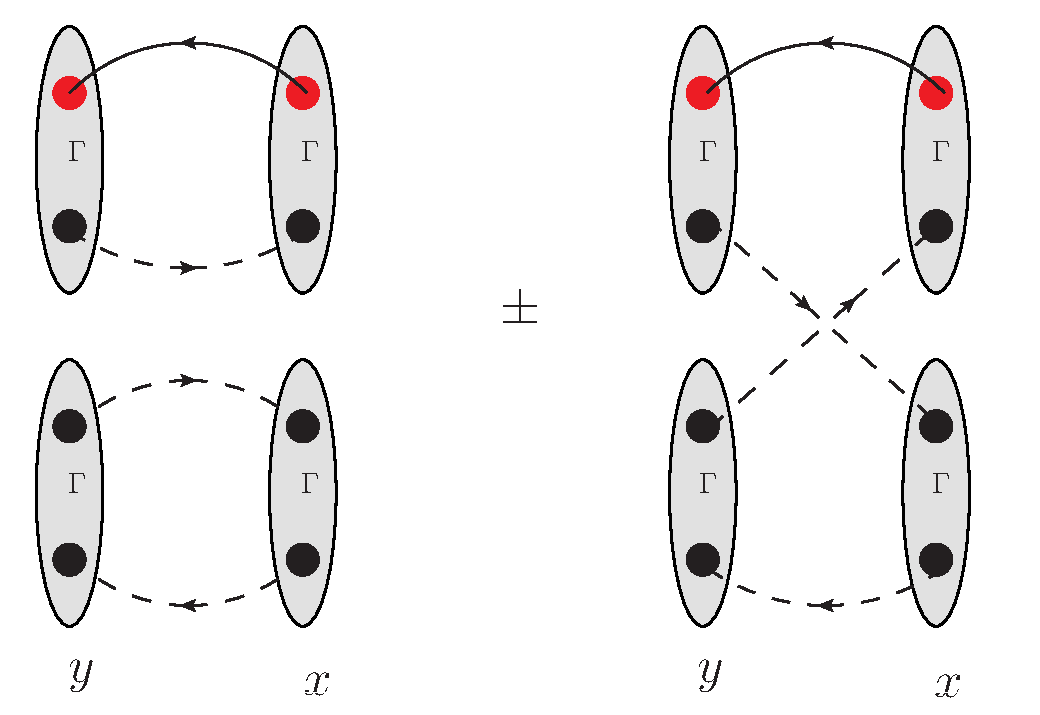
\includegraphics[width=.5\columnwidth]{contract1.eps}
\caption{The direct term (left) and exchange term (right) coming from the contractions given in Eqs.~\eqref{eqn:15 contraction} and~\eqref{eqn:6 contraction}.  The red dots and the solid black arrow refer to the charm quarks and their propgagator, respectively.  The remaining black dots and dashed lines are the SU(3) flavor symmetric quarks and their corresponding propagators. \label{fig:15 and 6}}
\end{figure}
The $[\bar{3}]$ case is difficult and highly non-trivial.  Performing the calculation \emph{by hand}, I find
\begin{multline}\label{eqn:3b contraction}
\langle O^{i}_{[\bar3]}\bar{O}^{i}_{[\bar3]}\rangle=\operatorname{Tr}[\left.\Gamma \gamma_{5} \mathcal{S}_{y^{\prime} ; x}^{\dagger} \gamma_{5} \Gamma \mathcal{S}_{y^{\prime} ; x}\right] \operatorname{Tr}\left[\Gamma \gamma_{5} \mathcal{S}_{y ; x}^{\dagger} \gamma_{5} \Gamma \mathcal{C}_{y ; x}\right]\\
+\frac{1}{3} \operatorname{Tr}\left[\Gamma \gamma_{5} \mathcal{S}_{y ; x}^{\dagger} \gamma_{5} \Gamma \gamma_{5} \mathcal{S}_{y^{\prime} ; x}^{\dagger} \gamma_{5} \Gamma \mathcal{S}_{y^{\prime} ; x} \Gamma \mathcal{C}_{y ; x}\right] 
-\frac{11}{12} \operatorname{Tr}\left[\Gamma \mathcal{S}_{x ; x} \Gamma \gamma_{5} \mathcal{S}_{y^{\prime} ; x}^{\dagger} \gamma_{5} \Gamma{ \color{red}\mathcal{S}_{y^{\prime} ; y} }\Gamma \mathcal{C}_{y ; x}\right]\\
-\frac{1}{12}\operatorname{Tr}\left[\Gamma \mathcal{S}_{x ; x}\right]\operatorname{Tr}\left[ \Gamma \gamma_{5} \mathcal{S}_{y^{\prime} ; x}^{\dagger} \gamma_{5} \Gamma {\color{red}\mathcal{S}_{y^{\prime} ; y} }\Gamma \mathcal{C}_{y ; x}\right]
-\frac{1}{12}\operatorname{Tr}\left[\Gamma {\color{red}\mathcal{S}_{y' ; y'}}\right]\operatorname{Tr}\left[ \Gamma \gamma_{5} \mathcal{S}_{y ; x}^{\dagger} \gamma_{5} \Gamma \mathcal{S}_{x ; x} \Gamma \mathcal{C}_{y ; x}\right]\\
-\frac{1}{4}\operatorname{Tr}\left[\Gamma \mathcal{S}_{x ; x}\right]\operatorname{Tr}\left[\Gamma {\color{red}\mathcal{S}_{y' ; y'}}\right]\operatorname{Tr}\left[ \Gamma \gamma_{5} \mathcal{S}_{y ; x}^{\dagger} \gamma_{5} \Gamma  \mathcal{C}_{y ; x}\right]
\end{multline}
%\begin{multline}\label{eqn:3b contraction}
%\langle O^{1}_{[\bar{3}]}(y',y)\bar{O}^{1}_{[\bar{3}]}(x,x)\rangle =\text{Tr}\left[\Gamma \gamma_5\mathcal{S}^\dag_{y'; x}\gamma_5\Gamma\mathcal{S}^{}_{y';x}\right]
%\text{Tr}\left[\Gamma \gamma_5\mathcal{S}^\dag_{y; x}\gamma_5\Gamma\mathcal{C}^{}_{y; x}\right]\\
%+\frac{1}{3}\text{Tr}\left[\Gamma \gamma_5\mathcal{S}^\dag_{y; x}\gamma_5\Gamma\gamma_5\mathcal{S}^\dag_{y'; x}\gamma_5\Gamma \mathcal{S}^{}_{y'; x}\Gamma\mathcal{C}^{}_{y; x}\right]\\
%-\frac{8}{3}\text{Tr}\left[\Gamma \mathcal{S}^{}_{x; x}\Gamma\gamma_5\mathcal{S}^\dag_{y'; x}\gamma_5\Gamma {\color{red}\mathcal{S}^{}_{y'; y}}\Gamma\mathcal{C}^{}_{y; x}\right]\ .
%\end{multline}
Note the terms in {\color{red}red}.  These terms are numerically problematic to calculate, as they in principle require an \emph{all-to-all} propagator\footnote{This assumes we want to do momentum projection at the sink.}.  As before, the remaining contractions in the $[\bar{3}]$ representation are identical due to SU(3) flavor symmetry. \autoref{fig:3b} shows this expression diagrammatically.

As a recap, I find the following expressions for the [15], [6], and [$\bar{3}$]:
{\tiny
\begin{displaymath}
\begin{matrix}
{\large\text{irrep}} & {\large\text{contraction}} \\
\hline
\hline
 [15]&\text{Tr}\left[\Gamma \gamma_5\mathcal{S}^\dag_{y';x}\gamma_5\Gamma\mathcal{S}^{}_{y';x}\right]
\text{Tr}\left[\Gamma \gamma_5\mathcal{S}^\dag_{y;x}\gamma_5\Gamma\mathcal{C}^{}_{y;x}\right]
-\text{Tr}\left[\Gamma \gamma_5\mathcal{S}^\dag_{y;x}\gamma_5\Gamma\mathcal{S}^{}_{y';x}\Gamma \gamma_5\mathcal{S}^\dag_{y';x}\gamma_5\Gamma\mathcal{C}^{}_{y;x}\right] \\
\hline
 [6]&\text{Tr}\left[\Gamma \gamma_5\mathcal{S}^\dag_{y';x}\gamma_5\Gamma\mathcal{S}^{}_{y';x}\right]
\text{Tr}\left[\Gamma \gamma_5\mathcal{S}^\dag_{y;x}\gamma_5\Gamma\mathcal{C}^{}_{y;x}\right]
+\text{Tr}\left[\Gamma \gamma_5\mathcal{S}^\dag_{y;x}\gamma_5\Gamma\mathcal{S}^{}_{y';x}\Gamma \gamma_5\mathcal{S}^\dag_{y';x}\gamma_5\Gamma\mathcal{C}^{}_{y;x}\right] \\
\hline
[\bar 3]&\text{Tr}[\left.\Gamma \gamma_{5} \mathcal{S}_{y^{\prime} ; x}^{\dagger} \gamma_{5} \Gamma \mathcal{S}_{y^{\prime} ; x}\right] \operatorname{Tr}\left[\Gamma \gamma_{5} \mathcal{S}_{y ; x}^{\dagger} \gamma_{5} \Gamma \mathcal{C}_{y ; x}\right]
+\frac{1}{3} \operatorname{Tr}\left[\Gamma \gamma_{5} \mathcal{S}_{y ; x}^{\dagger} \gamma_{5} \Gamma \gamma_{5} \mathcal{S}_{y^{\prime} ; x}^{\dagger} \gamma_{5} \Gamma \mathcal{S}_{y^{\prime} ; x} \Gamma \mathcal{C}_{y ; x}\right] \\
& 
-\frac{11}{12} \operatorname{Tr}\left[\Gamma \mathcal{S}_{x ; x} \Gamma \gamma_{5} \mathcal{S}_{y^{\prime} ; x}^{\dagger} \gamma_{5} \Gamma{ \color{red}\mathcal{S}_{y^{\prime} ; y} }\Gamma \mathcal{C}_{y ; x}\right]
-\frac{1}{12}\operatorname{Tr}\left[\Gamma \mathcal{S}_{x ; x}\right]\operatorname{Tr}\left[ \Gamma \gamma_{5} \mathcal{S}_{y^{\prime} ; x}^{\dagger} \gamma_{5} \Gamma {\color{red}\mathcal{S}_{y^{\prime} ; y} }\Gamma \mathcal{C}_{y ; x}\right]\\
&
-\frac{1}{12}\operatorname{Tr}\left[\Gamma {\color{red}\mathcal{S}_{y' ; y'}}\right]\operatorname{Tr}\left[ \Gamma \gamma_{5} \mathcal{S}_{y ; x}^{\dagger} \gamma_{5} \Gamma \mathcal{S}_{x ; x} \Gamma \mathcal{C}_{y ; x}\right]
-\frac{1}{4}\operatorname{Tr}\left[\Gamma \mathcal{S}_{x ; x}\right]\operatorname{Tr}\left[\Gamma {\color{red}\mathcal{S}_{y' ; y'}}\right]\operatorname{Tr}\left[ \Gamma \gamma_{5} \mathcal{S}_{y ; x}^{\dagger} \gamma_{5} \Gamma  \mathcal{C}_{y ; x}\right]\\
\hline
\end{matrix}
\end{displaymath}
}

\begin{figure}
\center
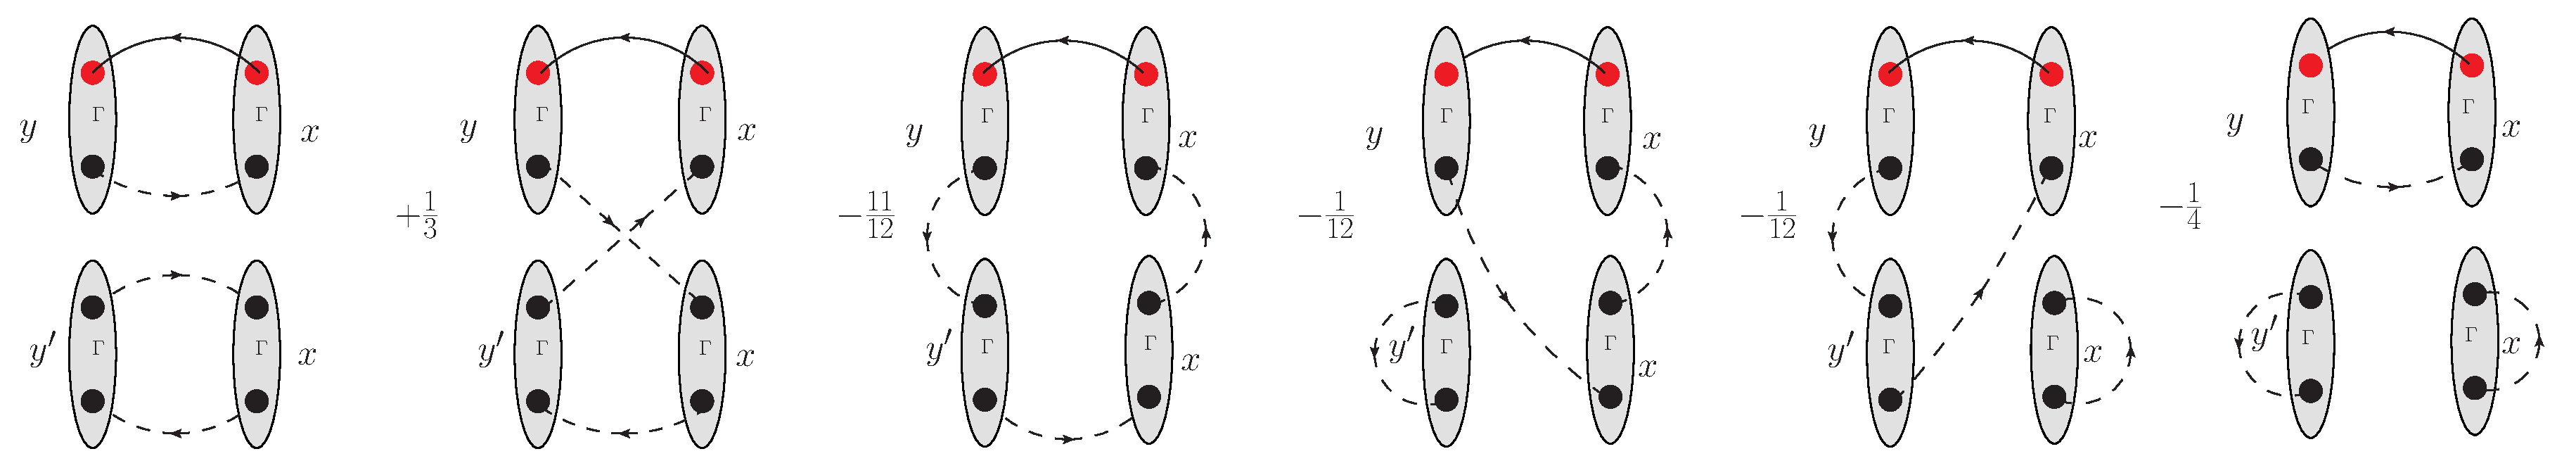
\includegraphics[width=\columnwidth]{contract3.eps}
\caption{The direct term (left), exchange term (next-to-left), and `disconnected' terms (everything else) coming from the contractions given in Eq.~\eqref{eqn:3b contraction}.  The red dots and the solid black arrow refer to the charm quarks and their propgagator, respectively.  The remaining black dots and dashed lines are the SU(3) flavor symmetric quarks and their corresponding propagators. \label{fig:3b}}
\end{figure}

\subsection{In the Isospin limit (2+1+1)}
Work in progress. . .

\subsection{Projecting onto zero momentum}
To project onto zero momentum, I sum over all possible sink locations $y$ and $y'$,
\begin{displaymath}
\frac{1}{|\Lambda_3|}\sum_{y,y'\in\Lambda_3}\langle O(y',y)\bar O(x,x)\rangle\ ,
\end{displaymath}
where $|\Lambda_3|$ is the lattice spatial dimension.


%\subsection{}

%\newpage
%\appendix

%\clearpage
%\bibliography{references}

\end{document}  
